
\begin{figure}[hpt!]

\centering
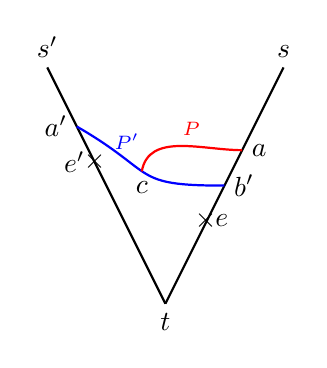
\begin{tikzpicture}[scale=1.5]

\definecolor{dgreen}{rgb}{0.0, 0.5, 0.0}
\begin{scope}[xshift=0cm]
\coordinate (s) at (-1,2);
\coordinate (s1) at (1,2);
\coordinate (t) at (0,0);
\coordinate (ts) at (0,0.4);
\coordinate (b1) at (0.5,1);

\coordinate (a1) at (-0.75,1.5);
\coordinate (a) at (0.65,1.3);
\coordinate (v) at (0.34,0.7);
\coordinate (v1) at (-0.6,1.2);
\coordinate (c) at (-0.2,1.12);

\draw[thick](s)--(t);
\draw[thick](s1)--(t);
\node[above] at (s){$s'$};
\node[above] at (s1){$s$};
\node[below] at (t){$t$};
\node[left] at (a1){$a'$};
\node[right] at (a){$a$};
\node[right] at (b1){$b'$};
\node[below] at (c){$c$};


\draw[blue,thick] (a1) to[out=330,in=180,distance=.8cm]
node[pos=0.3,above]
{\scriptsize  $P'$}  (b1);

\draw[red,thick] (a) to[out=180,in=80]
node[pos=0.4,above]
{\scriptsize  $P$}  (c);

\node at (v1){$\times$};
\node[left] at (v1){$e'$};

\node at (v){$\times$};
\node[right] at (v){$e$};

\end{scope}

\end{tikzpicture}

\caption{The bad case for us: $P' \in (>P)$ intersects with $P$ and then passes through the edge $e$ that $P$ avoids. }
\label{fig:multiple}
\end{figure}
